\chapter{Unconstrained Optimization}
\graphicspath{{../../img/img-2-3/}}

\section{Newton's and Gauss-Newton's Methods}

Following the discussion on gradient descent method, we still consider the 
unconstrained optimization problem (restated here in E.q. (\ref{uncstrn-opt})).

\begin{equation}
    \min_{\textbf{x}\in \mathbb{R}^d}{f(\textbf{x})}
    \label{uncstrn-opt}
\end{equation}

First we discuss the second-order method (Newton's method), which utilizes information
in the second-order derivatives. Then we focus on a certain type of objective function,
and approximate the hessian matrix in Newton's method by first-order derivatives.

% TODO: move this section to the example section
Here we compare the three optimization methods:

\begin{table}
    \begin{center}
        \caption{Comparison between three unconstrained optimization methods}

        \begin{tabular}{ |c|c|c| }
            \hline
            Optimization methods & Step size & Comments \\ 
            \hline
            Gradient descent & $\delta \textbf{x}_k = -\nabla f(\textbf{x}_k)$ & cell6 \\ 
            \hline
            Newton's method & $\delta \textbf{x}_k = 
            -[\nabla^2 f(\textbf{x}_k)]^{-1} \nabla f(\textbf{x}_k)$ & cell9 \\ 
            \hline
            Gauss-Newton's method & 
            \vtop{\hbox{\strut $\delta \textbf{x}_k = -\hat{H}^{-1} g$}
            \hbox{\strut $f(\textbf{x})=\frac{1}{2} \textbf{e}(\textbf{x})^T \textbf{e}(\textbf{x})$}
            \hbox{\strut $g = (\frac{\partial \textbf{e}(\textbf{x}_k)}{\partial \textbf{x}} 
            | _{\textbf{x}=\textbf{x}_k})^T$}
            \hbox{\strut $\hat{H} = g \cdot g^T$}
            }
            & cell12\\

            % Gauss-Newton's method & $\delta \textbf{x}_k = -\hat{H}^{-1} g$ \newline 
            % $f(\textbf{x})=\frac{1}{2} \textbf{e}(\textbf{x})^T \textbf{e}(\textbf{x})$ \newline 
            % $g = (\frac{\partial \textbf{e}(\textbf{x}_k)}{\partial \textbf{x}} 
            % | _{\textbf{x}=\textbf{x}_k})^T$ \newline 
            % $\hat{H} = g \cdot g^T$ & cell12\\
            \hline % \nabla 

        \end{tabular}
        
    \end{center}
\end{table}

\subsection{Newton's Method}
We approximate the objective function $f(\textbf{x})$ using Taylor's expansion:

\begin{equation}
    f(\textbf{x}_k+\delta \textbf{x}) \approx f(\textbf{x}_k) + 
    (\frac{\partial f(\textbf{x})}{\partial \textbf{x}} |_{\textbf{x}=\textbf{x}_k})
    \delta \textbf{x} +
    \frac{1}{2}\delta \textbf{x}^T (\frac{\partial^2 f(\textbf{x})}
    {\partial \textbf{x} \partial \textbf{x}^T}|_{\textbf{x}=\textbf{x}_k})
    \delta \textbf{x}
    \label{newton}
\end{equation}

where $\delta \textbf{x}$ is a small change on $\textbf{x} = \textbf{x}_k$. Here we define:

\begin{equation}
    q(\delta \textbf{x}, \textbf{x}_k) := 
    f(\textbf{x}_k) + 
    (\frac{\partial f(\textbf{x})}{\partial \textbf{x}} |_{\textbf{x}=\textbf{x}_k})
    \delta \textbf{x} +
    \frac{1}{2}\delta \textbf{x}^T (\frac{\partial^2 f(\textbf{x})}
    {\partial \textbf{x} \partial \textbf{x}^T}|_{\textbf{x}=\textbf{x}_k})
    \delta \textbf{x}
    \label{q}
\end{equation}

$q(\delta \textbf{x}, \textbf{x}_k)$ is a quadratic approximation of $f(\textbf{x})$
around $\textbf{x} = \textbf{x}_k$. Minimizing $q(\delta \textbf{x}, \textbf{x}_k)$
leads us to a descent direction (with step size indicated as well).
Then we can write the optimization problem of minimizing $q$:

\begin{equation}
    \min_{\delta \textbf{x} \in \mathbb{R}^d}{q(\delta \textbf{x}, \textbf{x}_k)}
\end{equation}

This is an unconstrained optimization problem and the objective function $q$ is quadratic 
and thus convex. $\delta \textbf{x}$ can be determined by setting the derivative of $q$ with respect
to $\delta \textbf{x}$ to zero:

\begin{equation}
    0=\frac{\partial q\left(\delta \mathbf{x}, \mathbf{x}_k\right)}{\partial \delta \mathbf{x}}=\nabla f\left(\mathbf{x}_k\right)^{\top}+\delta \mathbf{x}^{\top} \nabla^2 f\left(\mathbf{x}_k\right)
    \label{newton2}
\end{equation}

Recall the properties of a hessian matrix $H := \nabla^2 f(\mathbf{x})$:
\begin{enumerate}
    \item (For all twice differentiable functions,) $H$ is symmetric since $\frac{\partial f}{\partial x_i \partial x_j} = \frac{\partial f}{\partial x_j \partial x_i}$;
    \item (For convex functions,) $H$ is positive semi-definite; (See the proof \href{chrome-extension://efaidnbmnnnibpcajpcglclefindmkaj/https://wiki.math.ntnu.no/_media/tma4180/2016v/note2.pdf}{here}.)
    \item (For strictly convex functions,) $H$ is positive definite.
\end{enumerate}

Then we can solve E.q. \ref{newton2} uniquely \red{for $f(\textbf{x})$ being strictly convex} (i.e., 
$\nabla^2 f(\textbf{x}_k)\succ 0$):

\begin{equation}
    \delta \mathbf{x}=-\left[\nabla^2 f\left(\mathbf{x}_k\right)\right]^{-1} \nabla f\left(\mathbf{x}_k\right)
\end{equation}

Finally, we have the update function in Newton's method:

\begin{equation}
    \mathbf{x}_{k+1}=\mathbf{x}_k-\alpha_k\left[\nabla^2 f\left(\mathbf{x}_k\right)\right]^{-1} \nabla f\left(\mathbf{x}_k\right), \quad \alpha_k>0
    \label{update-newton}
\end{equation}

Fig. \ref{fig:y_2_3_1} is a graphic illustration on how we apply Newton's method. In each iteration 
$\mathbf{x} = \mathbf{x}^{(k)}$, we approximate $f(\mathbf{x})$ locally by a quadratic function
(drawn in the black line). In each step of applying the update equation (E.q. \ref{update-newton}),
we decide $\mathbf{x}^{(k+1)}$ by the minimizer given from $q(\delta \mathbf{x}, \mathbf{x}^{(k)})$.
Finally, it converges to a local minimum $f(\mathbf{x}^*)$.

\begin{figure}[!htb]
    \centering
    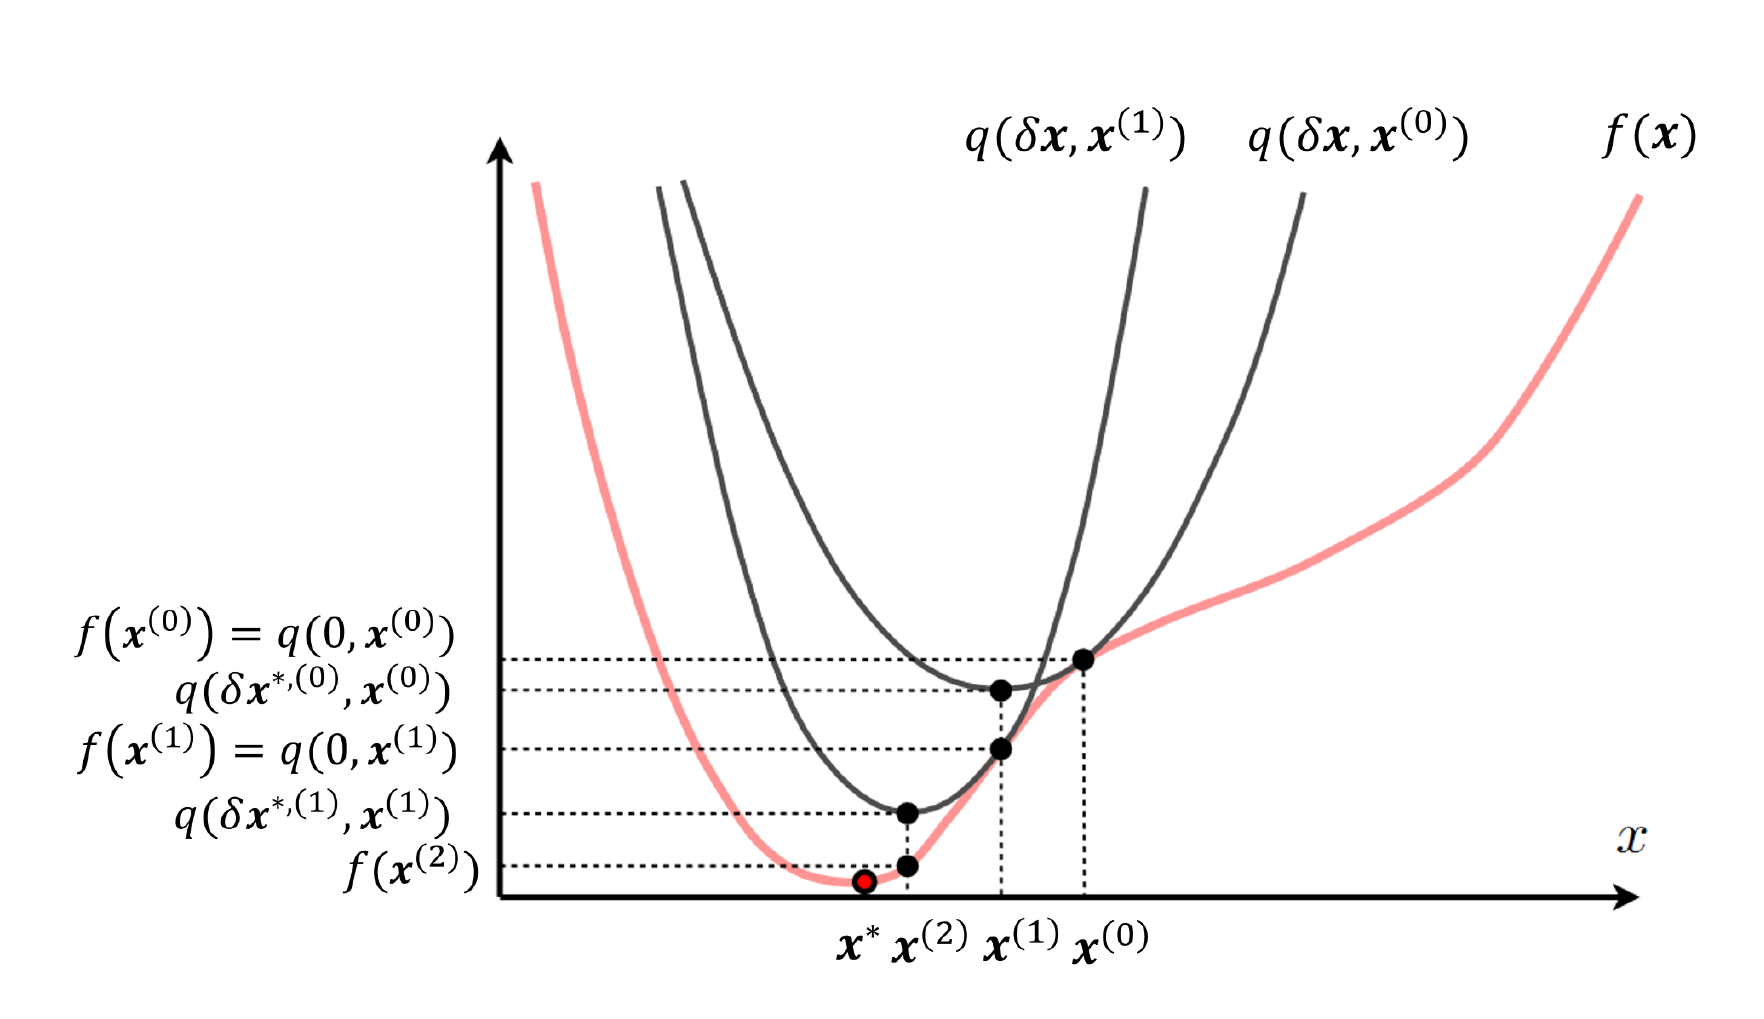
\includegraphics[width=10cm]{./img/img-2-3/y_2_3_1.png}
    \caption{Graphic illustration of the quadratic approximation in Newton's method}
    \label{fig:y_2_3_1}
\end{figure}

Here are some facts about Newton's method covered in the lecture slides.

\begin{figure}[!htb]
    \centering
    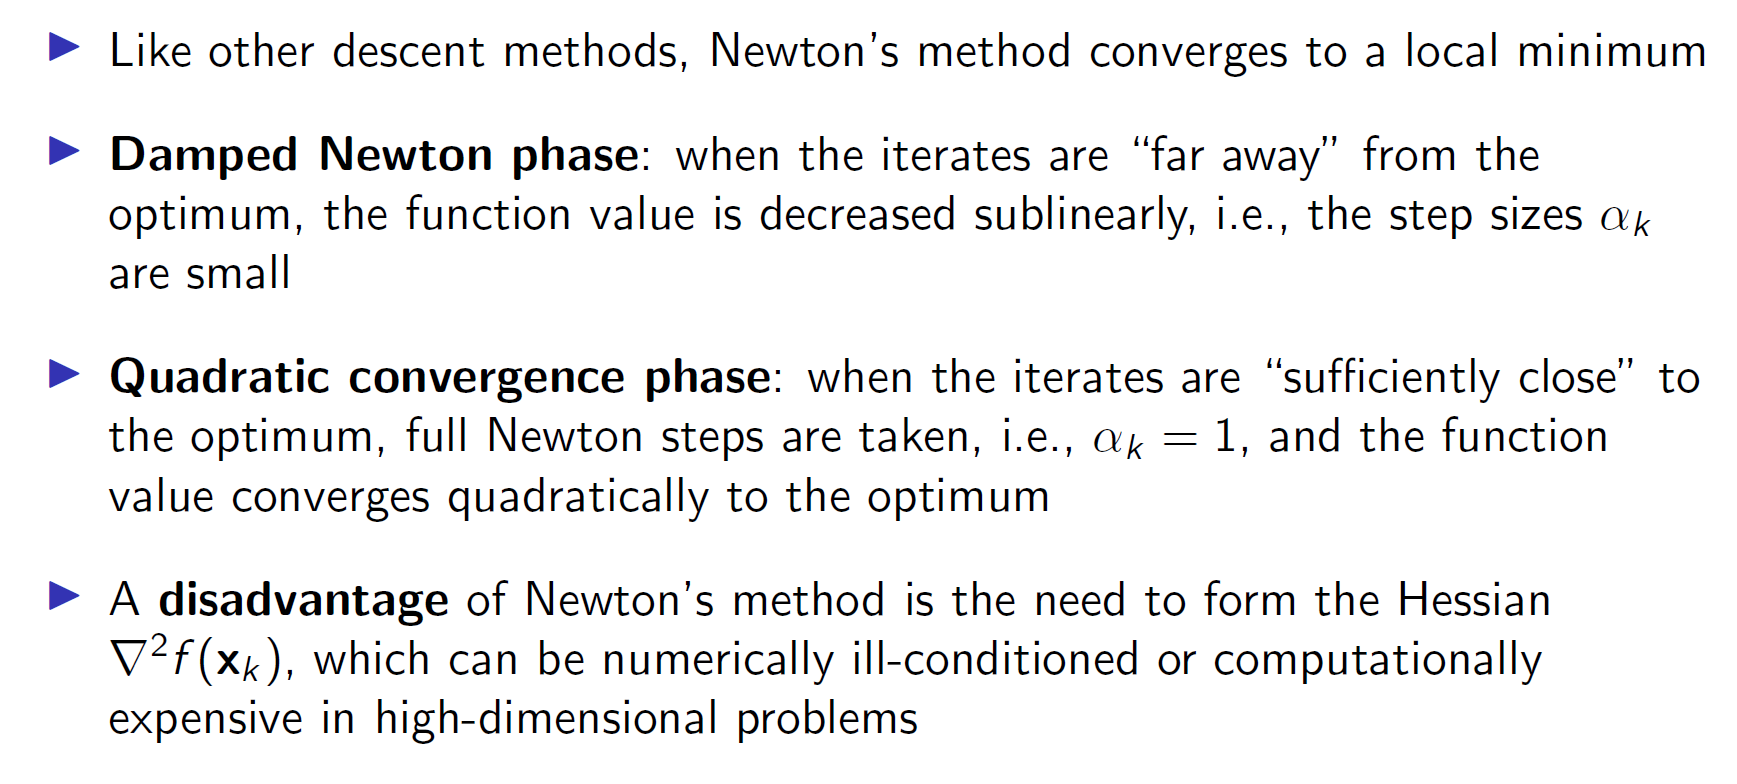
\includegraphics[width=12cm]{./img/img-2-3/y_2_3_2.png}
    % \caption{}
    \label{fig:y_2_3_2}
\end{figure}

Now Gauss-Newton's method comes into the picture as we want to bypass 
the above disadvantage of Newton's method (needs to compute $H$ and its inverse).

\subsection{Gauss-Newton's Method}

\textbf{Gauss-Newton} is an \textit{approximation} to Newton's method that avoids
computing the Hessian. It is applicable when the objective function has the
following quadratic form:

\begin{equation}
    f(\mathbf{x})=\frac{1}{2} \mathbf{e}(\mathbf{x})^{\top} \mathbf{e}(\mathbf{x}) \quad \mathbf{e}(\mathbf{x}) \in \mathbb{R}^m
\end{equation}

i.e., $f(\mathbf{x})= \frac{1}{2} \Vert \mathbf{e}(\mathbf{x}) \Vert _2^2 $.

To derive the Gauss-Newton's method, we first take a look at the derivative and hessian of $f(\mathbf{x})$:

\begin{figure}[!htb]
    \centering
    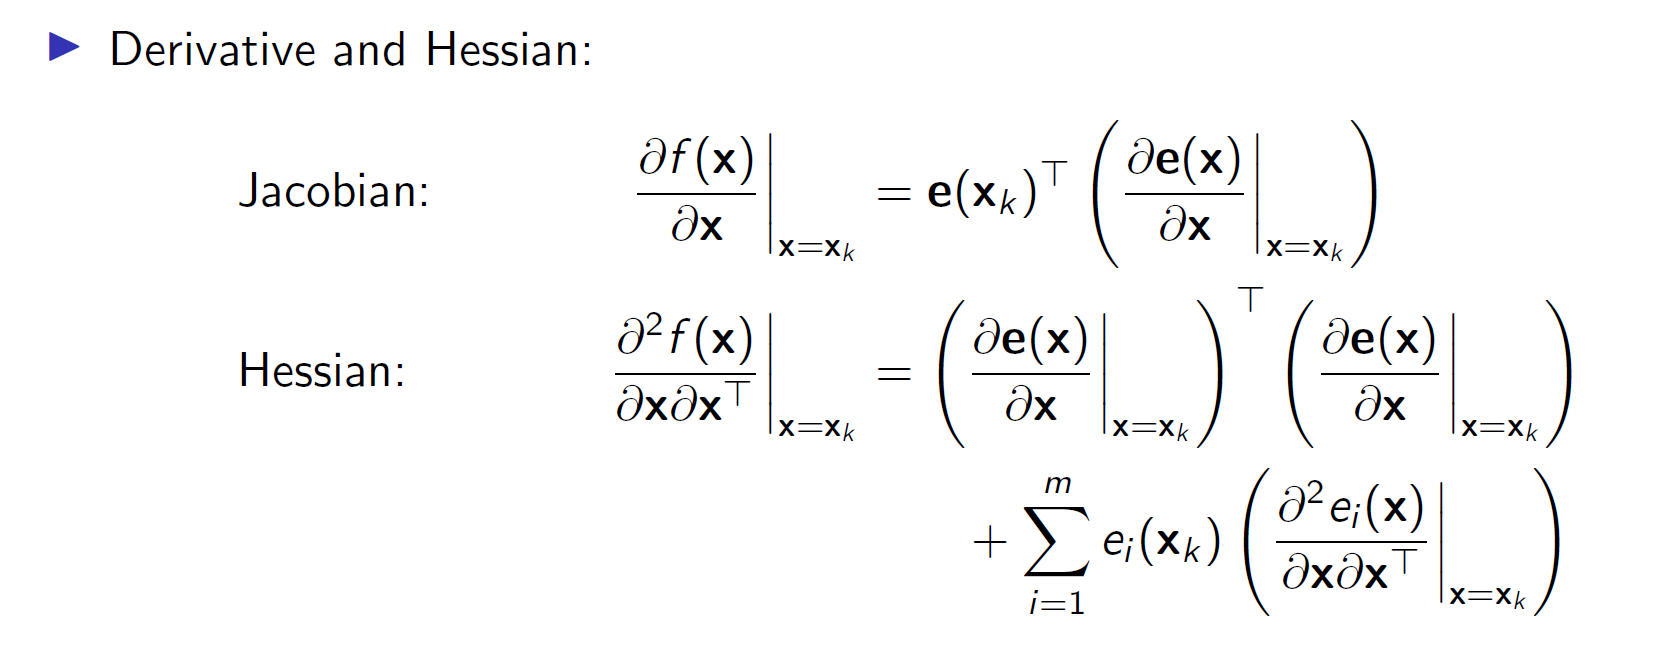
\includegraphics[width=12cm]{./img/img-2-3/y_2_3_3.png}
    % \caption{}
    \label{fig:y_2_3_3}
\end{figure}

Now, the second-order derivative only exists in the second term in hessian.
We assume the second term is small relative to the first and approximate hessian without second derivatives:

\begin{equation}
    \left.\frac{\partial^2 f(\mathbf{x})}{\partial \mathbf{x} \partial \mathbf{x}^{\top}}\right|_{\mathbf{x}=\mathbf{x}_k} \approx\left(\left.\frac{\partial \mathbf{e}(\mathbf{x})}{\partial \mathbf{x}}\right|_{\mathbf{x}=\mathbf{x}_k}\right)^{\top}\left(\left.\frac{\partial \mathbf{e}(\mathbf{x})}{\partial \mathbf{x}}\right|_{\mathbf{x}=\mathbf{x}_k}\right)
    \label{hessian-appr}
\end{equation}

To derive the update function, the rest procedure is basically the same as Newton's method, except for
we replace hessian in E.q. \ref{q} by E.q. \ref{hessian-appr}.
This leads to the update function in Gauss-Newton's method:

\begin{equation}
    \mathbf{x}_{k+1}=\mathbf{x}_k+\alpha_k \delta \mathbf{x}, \quad \alpha_k>0
\end{equation}

where $\delta \mathbf{x}$ can be determined from:

\begin{equation}
    \left(\left.\frac{\partial \mathbf{e}(\mathbf{x})}{\partial \mathbf{x}}\right|_{\mathbf{x}=\mathbf{x}_k}\right)^{\top}\left(\left.\frac{\partial \mathbf{e}(\mathbf{x})}{\partial \mathbf{x}}\right|_{\mathbf{x}=\mathbf{x}_k}\right) \delta \mathbf{x}=-\left(\left.\frac{\partial \mathbf{e}(\mathbf{x})}{\partial \mathbf{x}}\right|_{\mathbf{x}=\mathbf{x}_k}\right)^{\top} \mathbf{e}\left(\mathbf{x}_k\right)
    \label{gauss-newton-deltax}
\end{equation}

\textbf{Levenberg-Marquardt's Method}

The Levenberg-Marquardt's Method is a modified version of the Gauss-Newton's method 
to compensate the missing hessian term. The modification is based on E.q. \ref{gauss-newton-deltax},
which uses a positive diagonal matrix $D$:

\begin{equation}
    \left(\left.\frac{\partial \mathbf{e}(\mathbf{x})}{\partial \mathbf{x}}\right|_{\mathbf{x}=\mathbf{x}_k}\right)^{\top}\left(\left.\frac{\partial \mathbf{e}(\mathbf{x})}{\partial \mathbf{x}}\right|_{\mathbf{x}=\mathbf{x}_k} \red{+ \lambda D} \right) \delta \mathbf{x}=-\left(\left.\frac{\partial \mathbf{e}(\mathbf{x})}{\partial \mathbf{x}}\right|_{\mathbf{x}=\mathbf{x}_k}\right)^{\top} \mathbf{e}\left(\mathbf{x}_k\right)
    % \label{gauss-newton-deltax}
\end{equation}

When $\lambda \geq 0$ is large, the descent direction $\delta \mathbf{x}$ corresponds to a small step in
the direction of the steepest descent. This helps when the Hessian approximation
is poor or poorly conditioned by providing a meaningful direction.
An example choice of $D$:

\begin{equation}
    D = \textbf{diag}(\sum_{j}{J_j(\textbf{x}_k)^T J_j(\textbf{x}_k)})
\end{equation}

where $J_j(\textbf{x}) := \frac{\partial \textbf{e}_j(\textbf{x})}{\partial \textbf{x}} 
\in \mathbb{R}^{m_j \times n}, \lambda \geq 0, D \in \mathbb{R}^{n \times n}$.

\subsection{Example}

%TODO: example

